\subsection{پیاده‌سازی کنترل کننده LQR بر رویه کانال پیچ}
در بخش
\ref{quadchanell_roll}
شبیه‌سازی کانال رول استند چهارپره انجام شد. در این بخش به بررسی عملکرد چهارپره در حضور کنترل‌کننده LQR پرداخته می‌شود. در شبیه‌سازی برای بهینه‌سازی ضرایب وزنی از روش
TCACS \cite{Karimi2010}
استفاده شده است.
\begin{figure}[H]\label{lqr_roll_fig}
	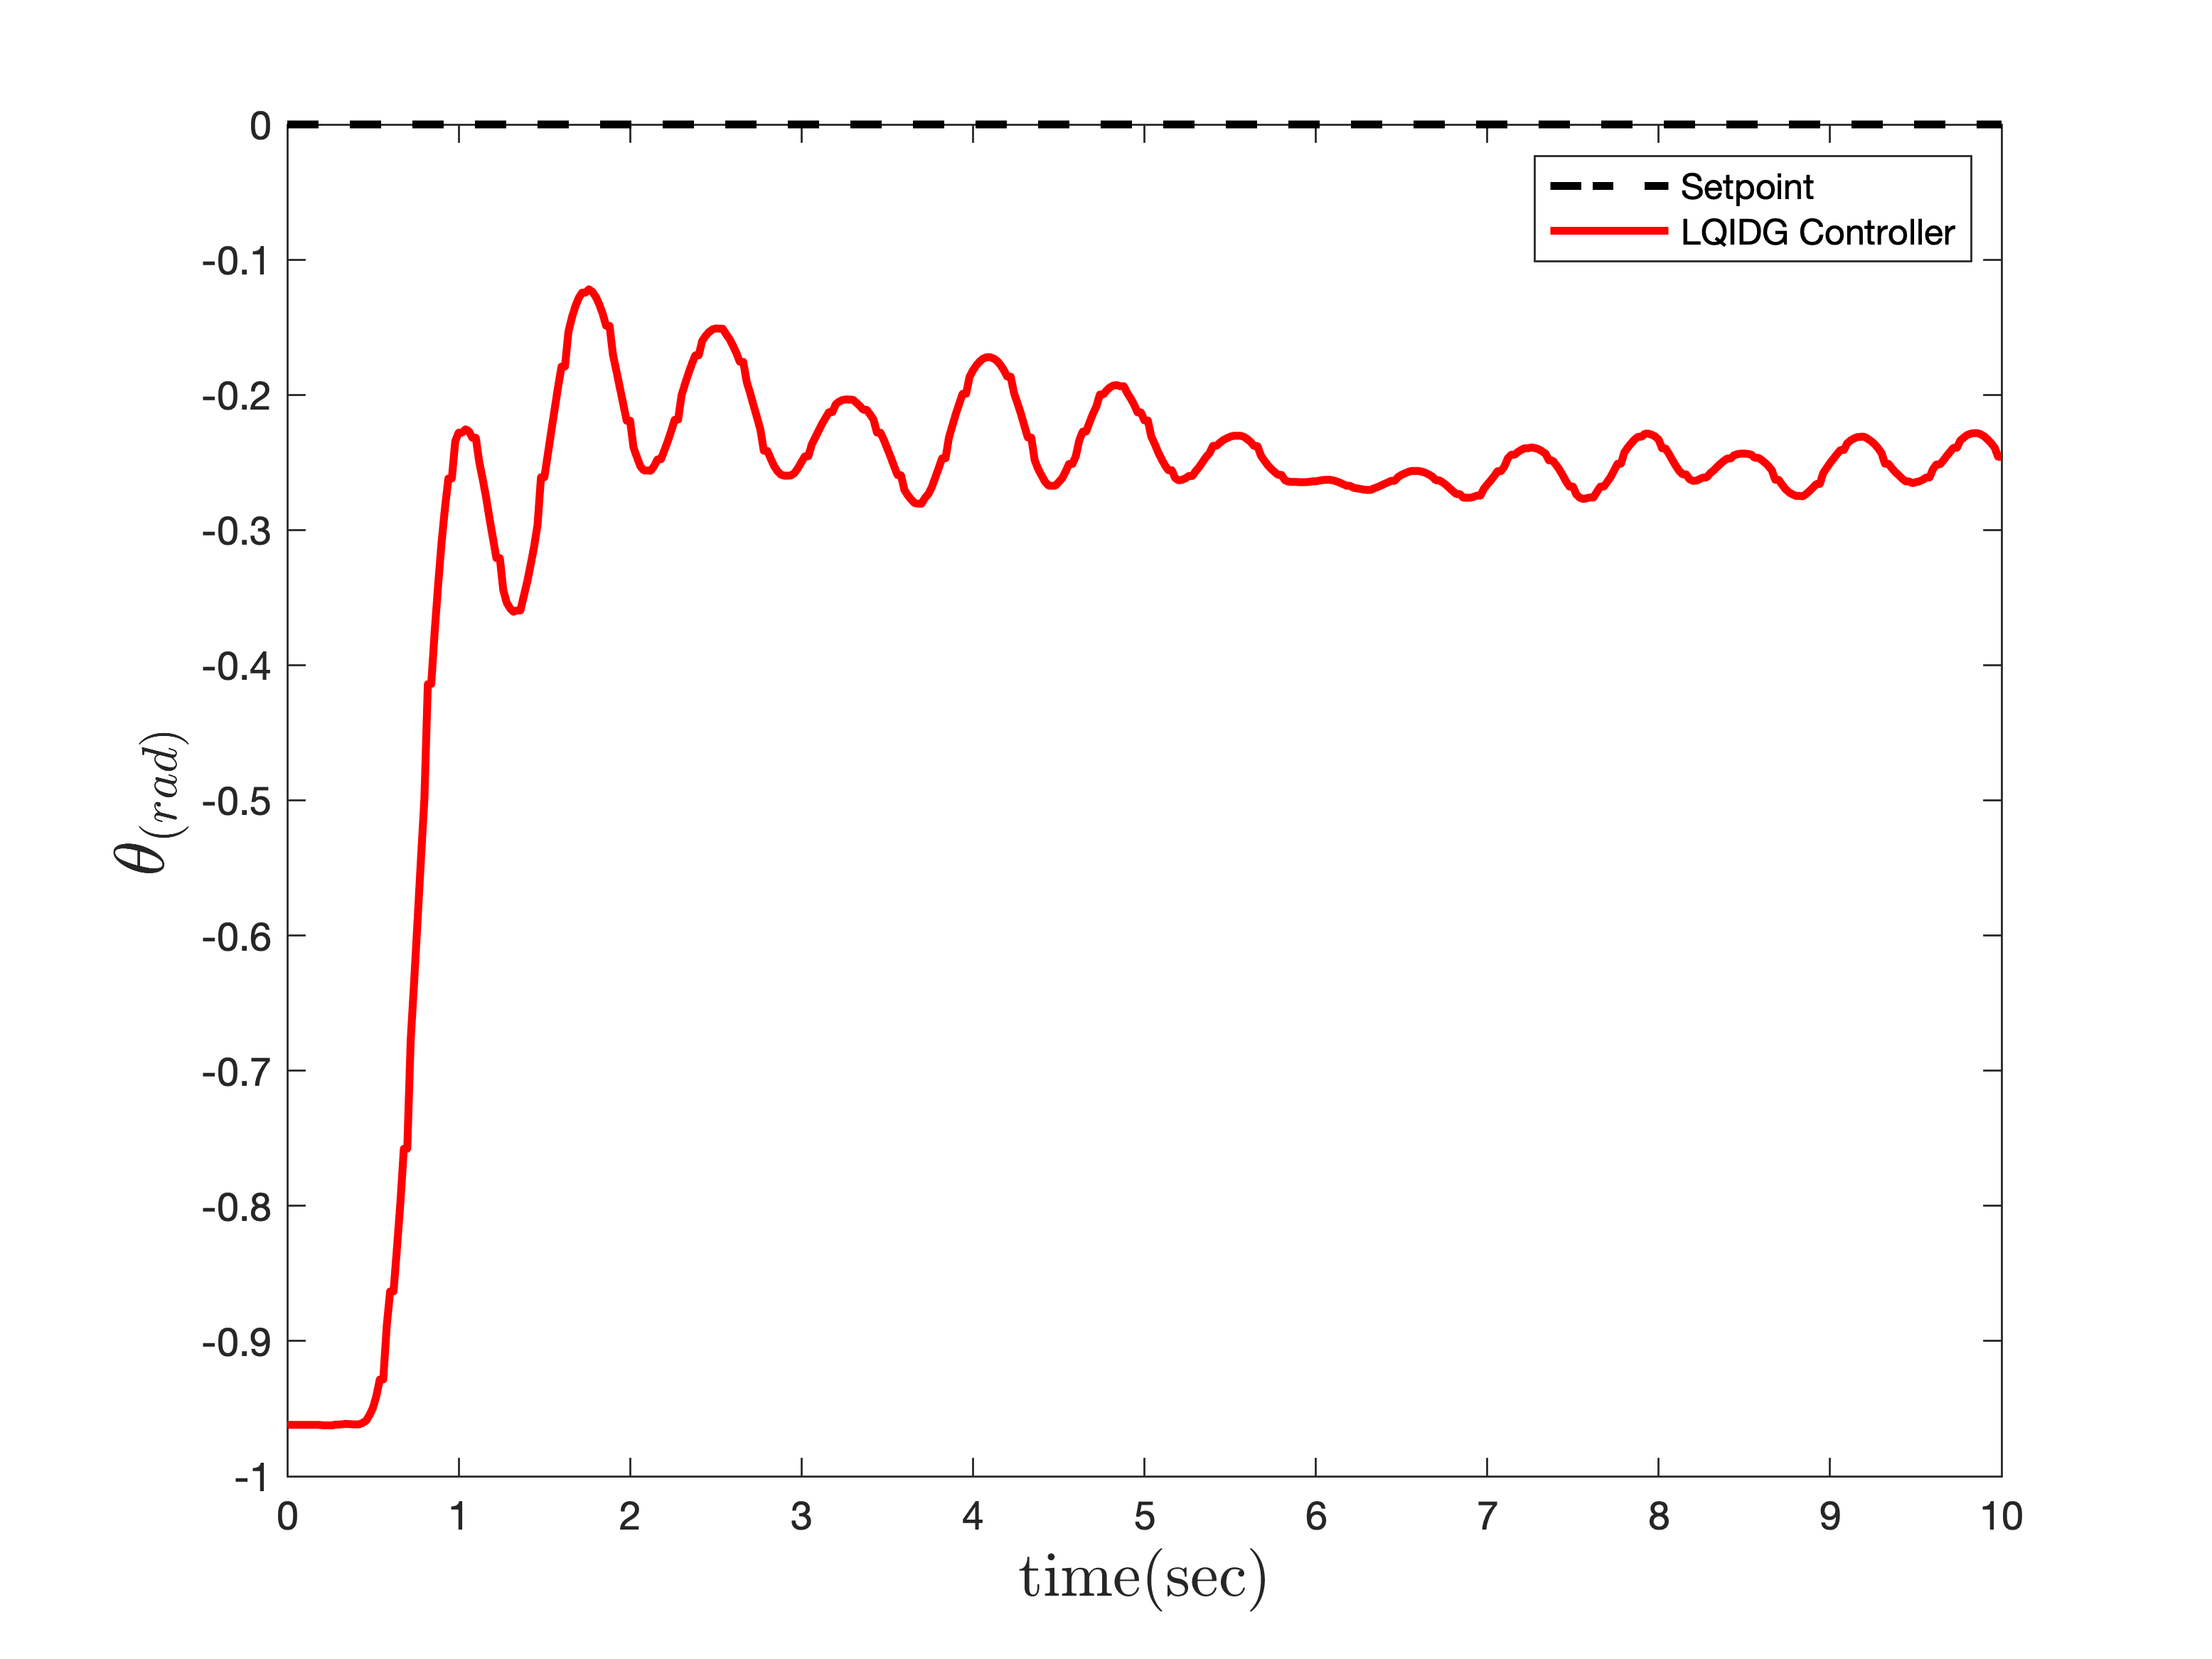
\includegraphics[width=.55\linewidth]{../Figures/Calibration/LQR/Pitch/lqr_pitch.png}
	\centering
	\caption{عملكرد LQR در کنترل زاويه رول (تعقیب ورودی صفر)}
\end{figure}
%
%\begin{figure}[H]
%	[width=12cm]
%	\centering
%	\begin{subfigure}
%		\centering
%		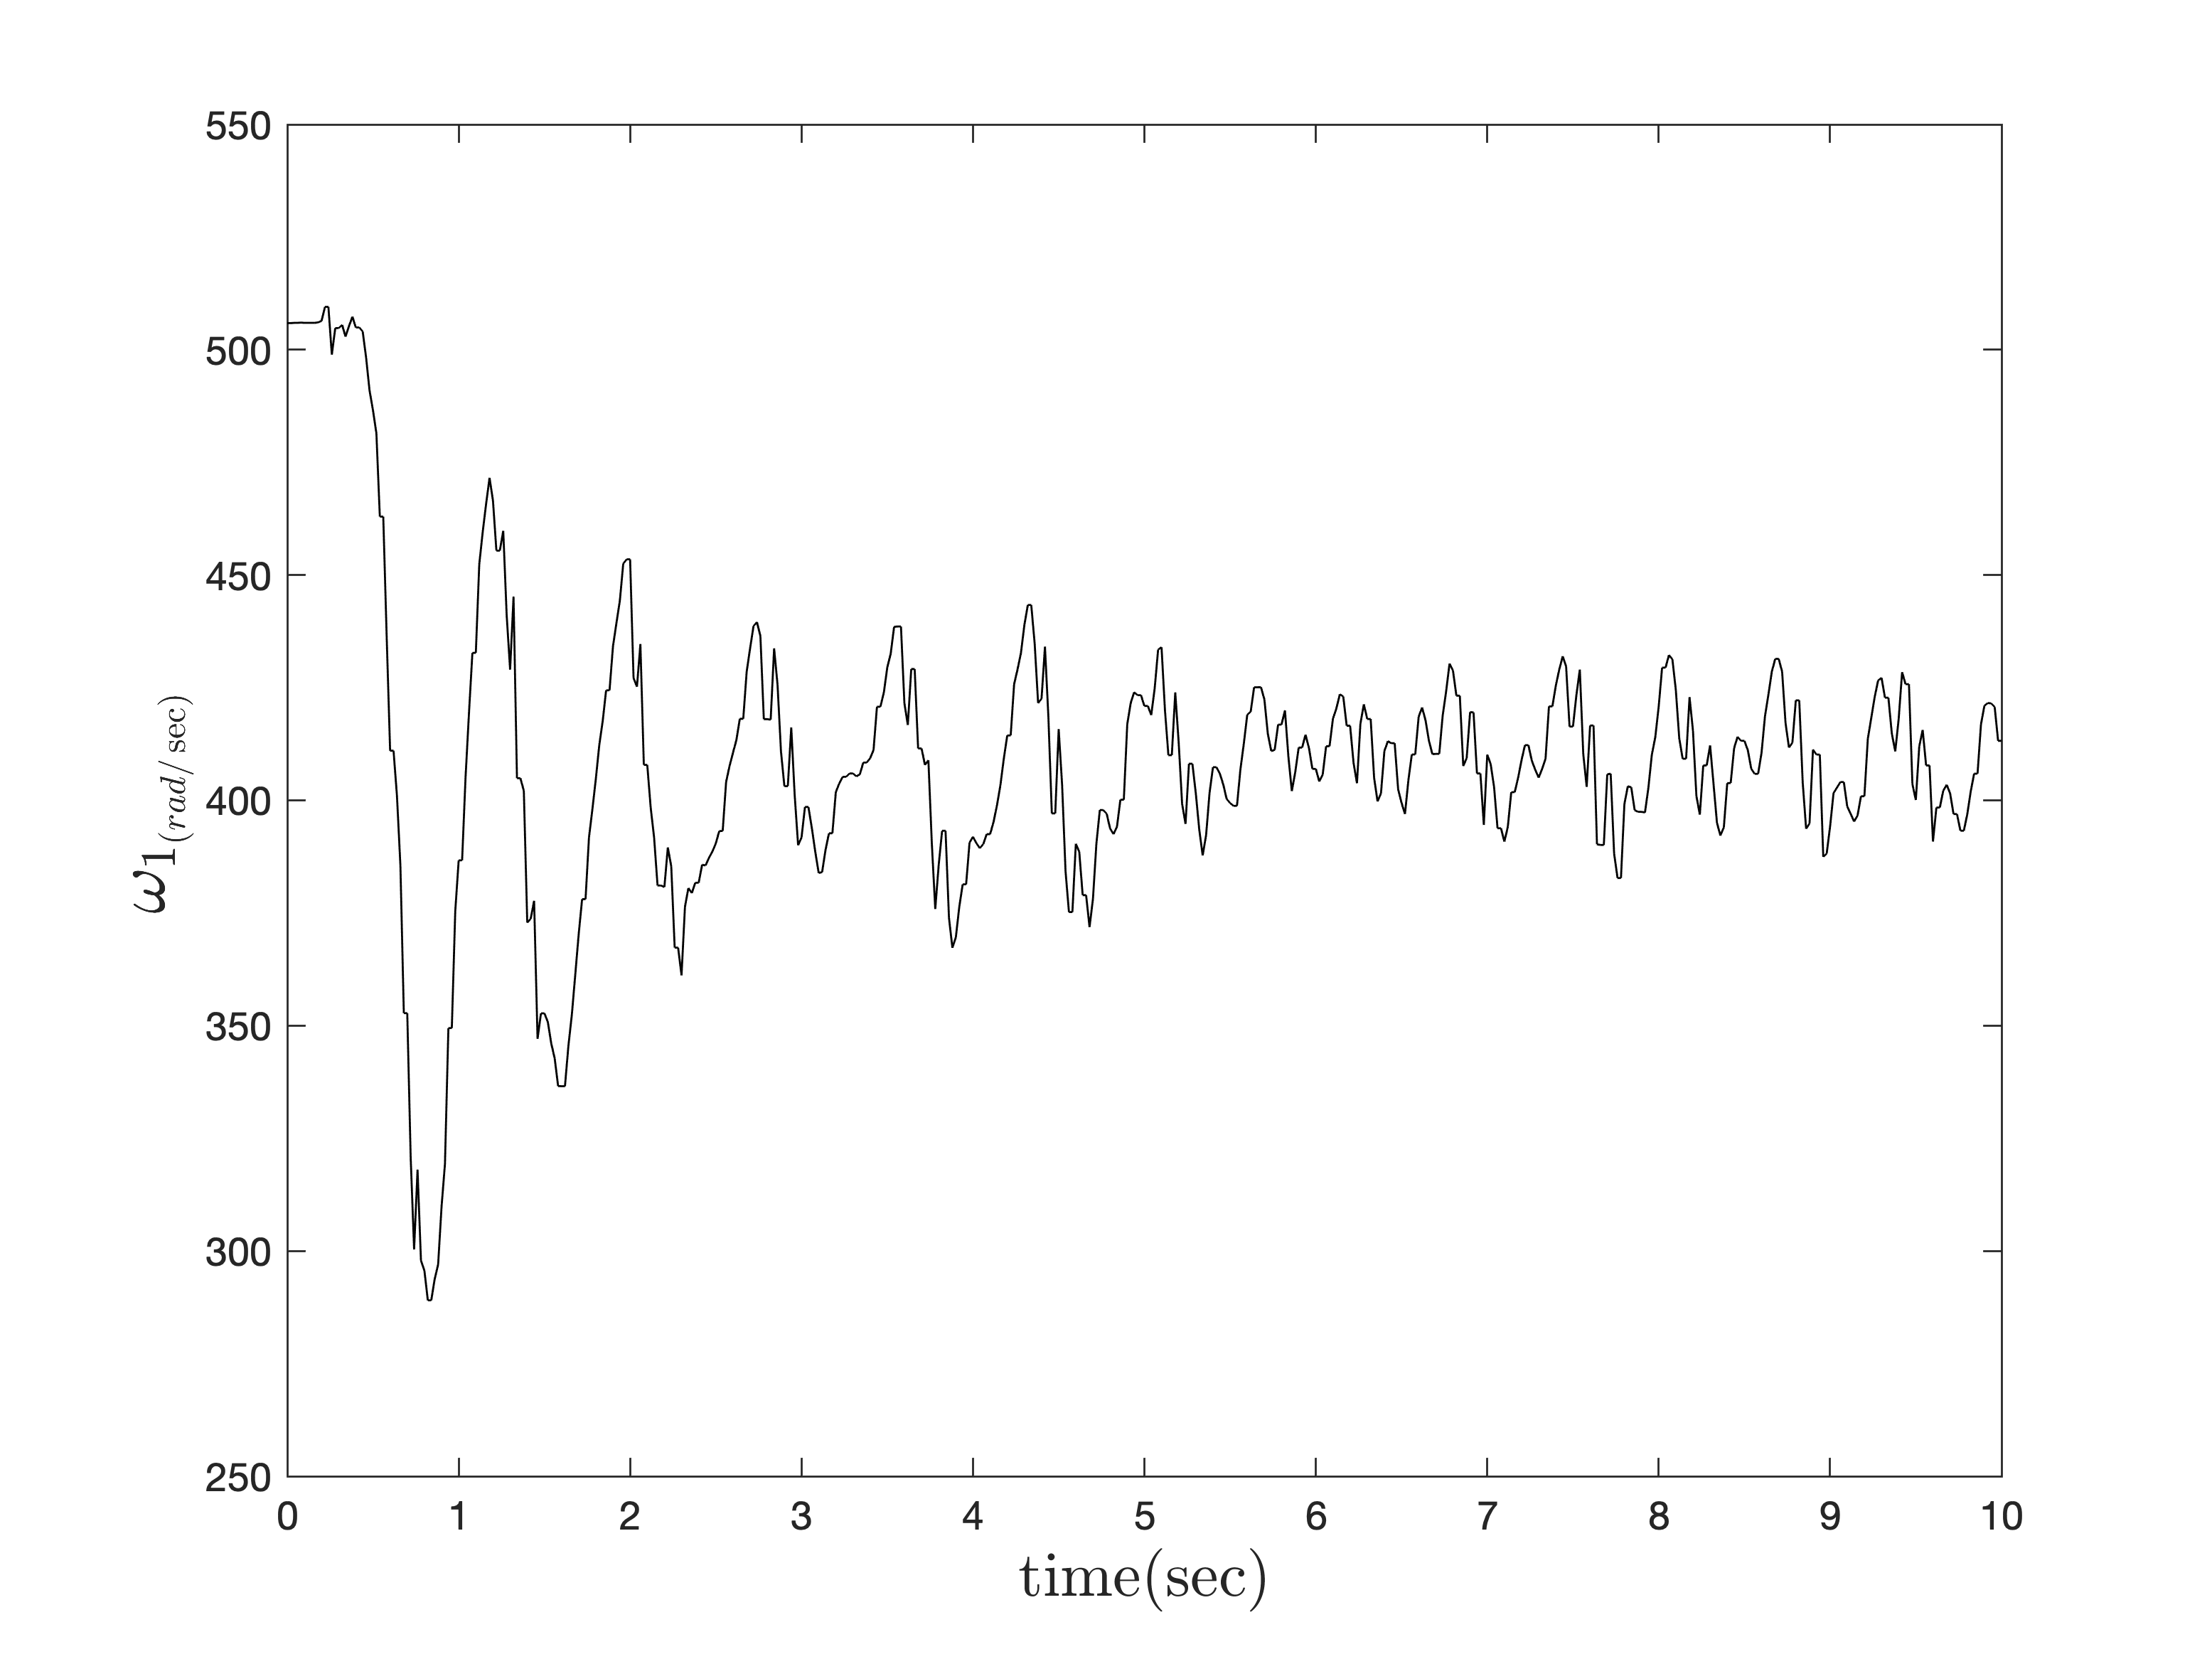
\includegraphics[width=12cm]{../Figures/Calibration/LQR/Pitch/lqr_pitch_Omega_1.png}
%		\caption{موتور شماره یک}
%	\end{subfigure}
%	\begin{subfigure}
%		\centering
%		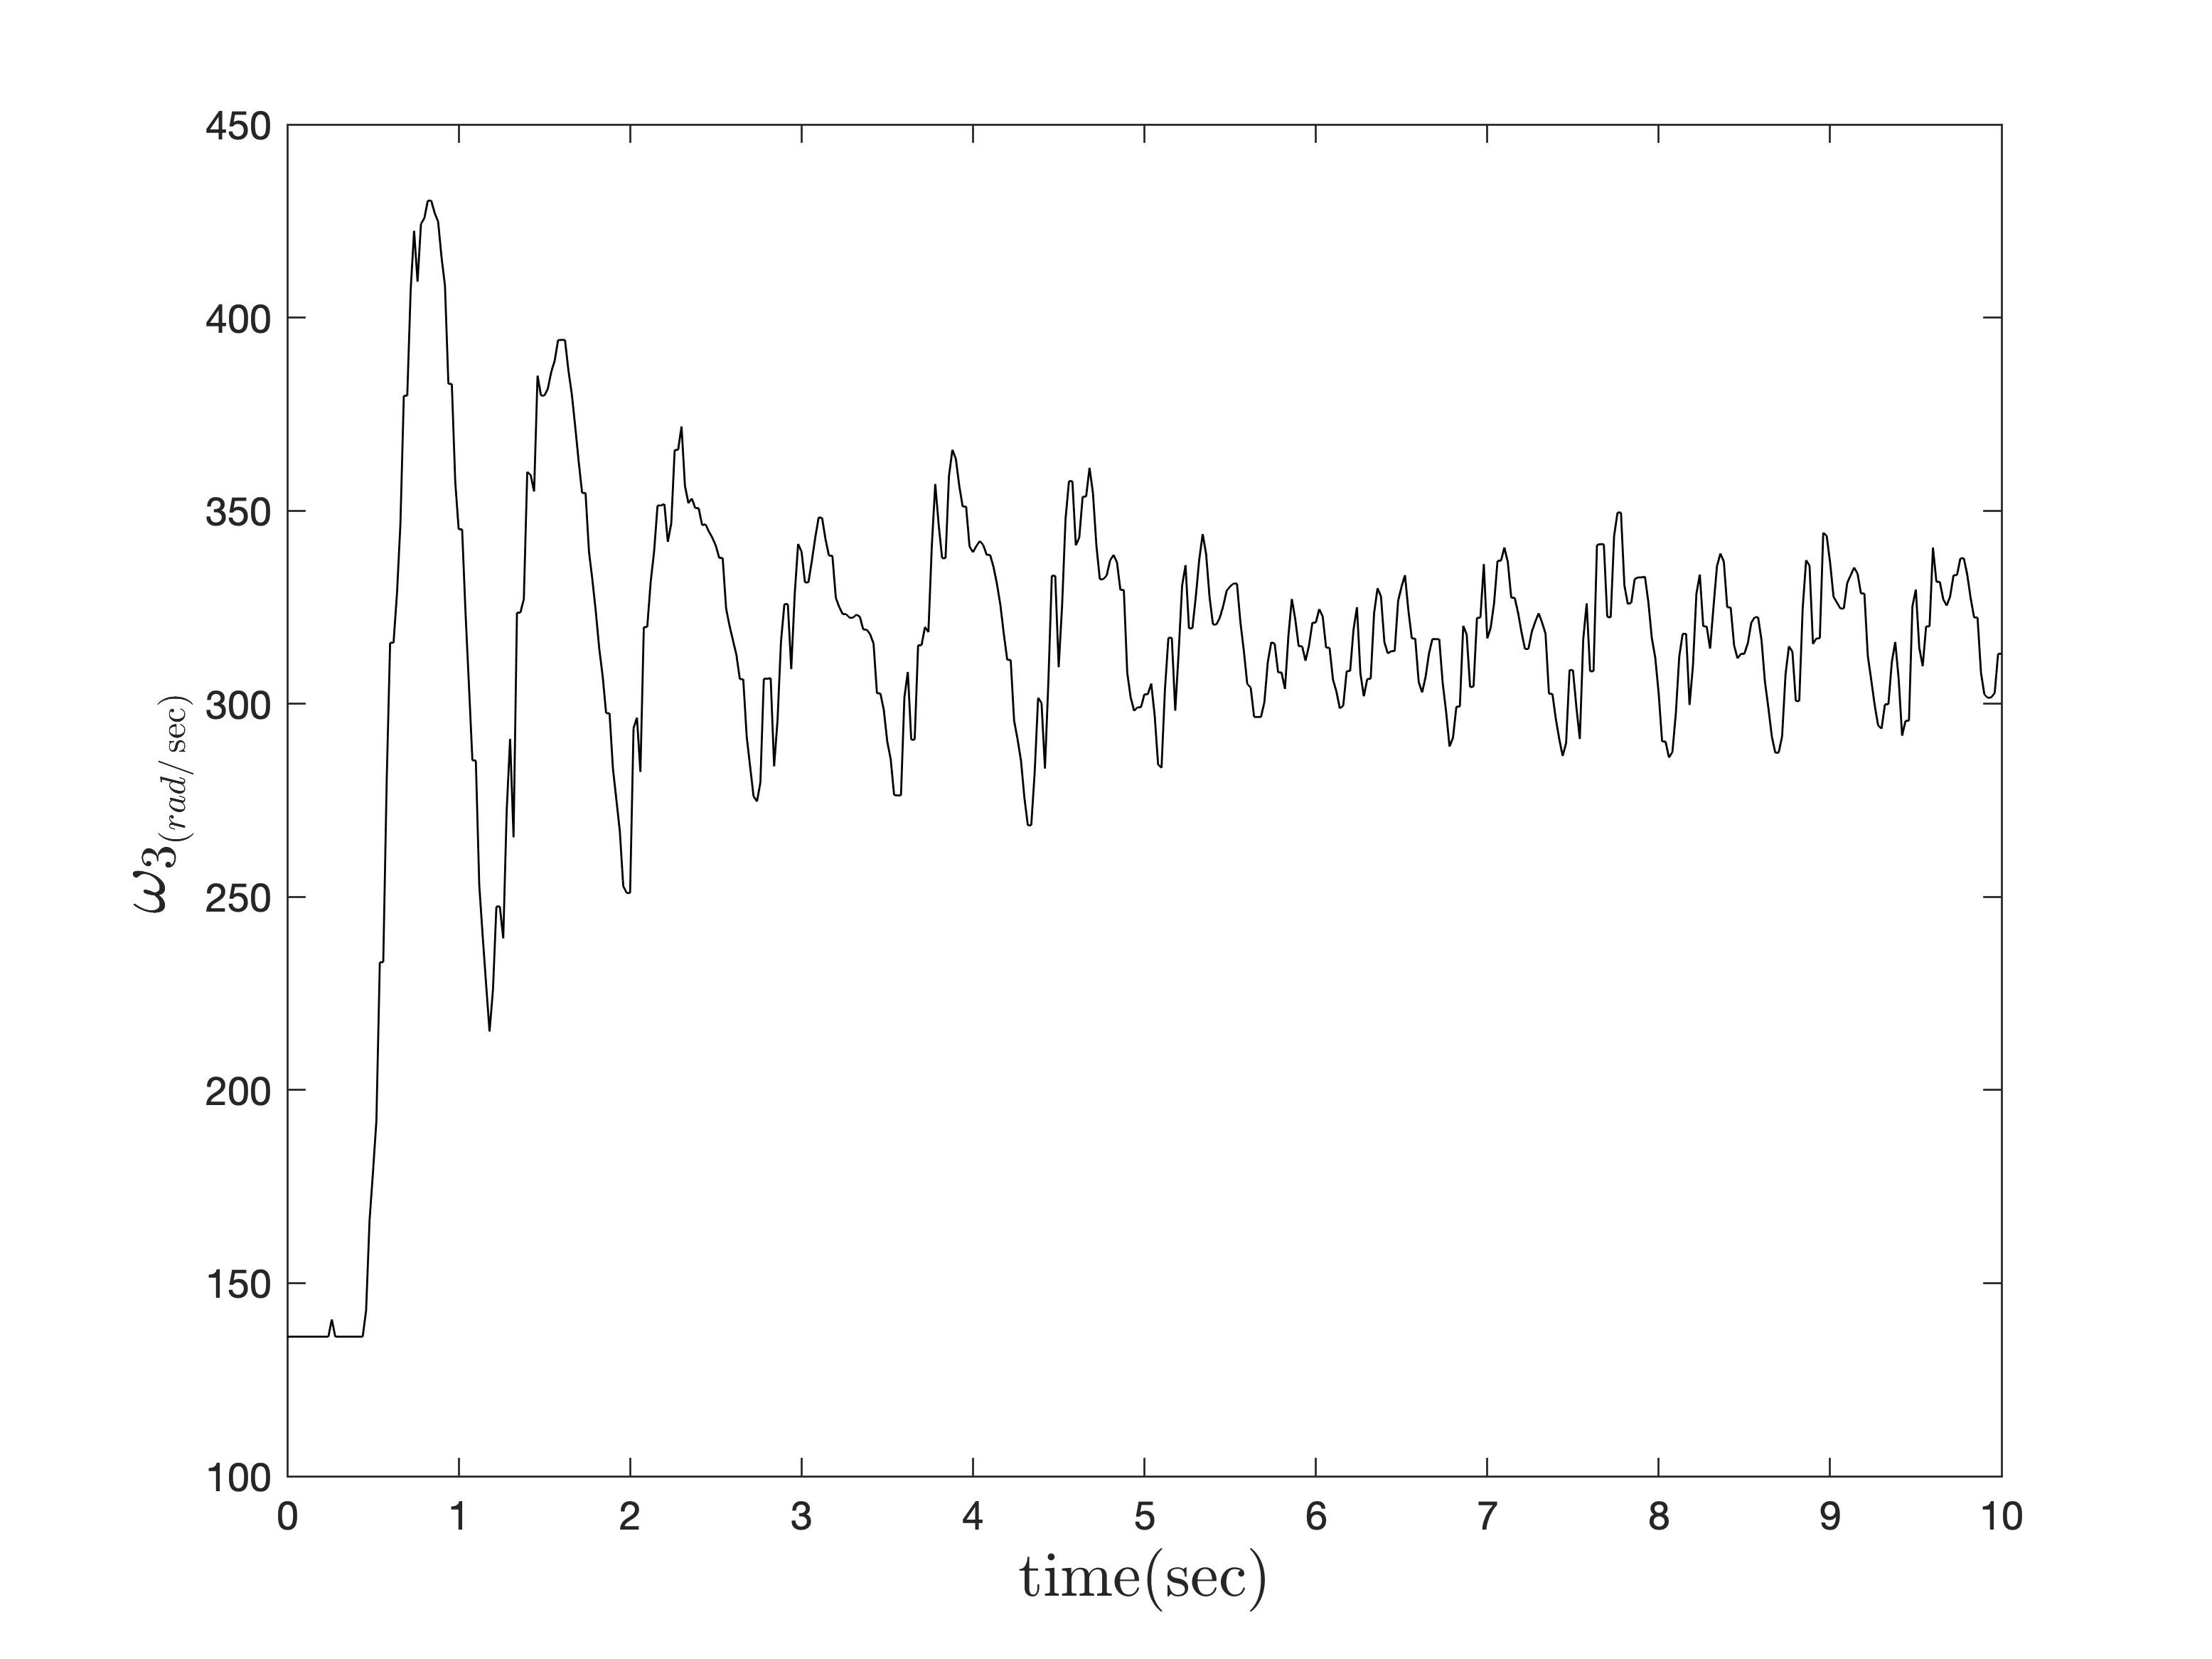
\includegraphics[width=12cm]{../Figures/Calibration/LQR/Pitch/lqr_pitch_Omega_3.png}
%		\caption{موتور شماره سه}
%	\end{subfigure}
%	\caption{‫‪فرمان کنترل‌کننده موتور سه و چهار در کنترل زاویه رول و پیچ (تعقیب ورودی صفر)}
%\end{figure}
\begin{figure}[H]
	\centering
	\subfigure[موتور شماره یک]{
		\centering
		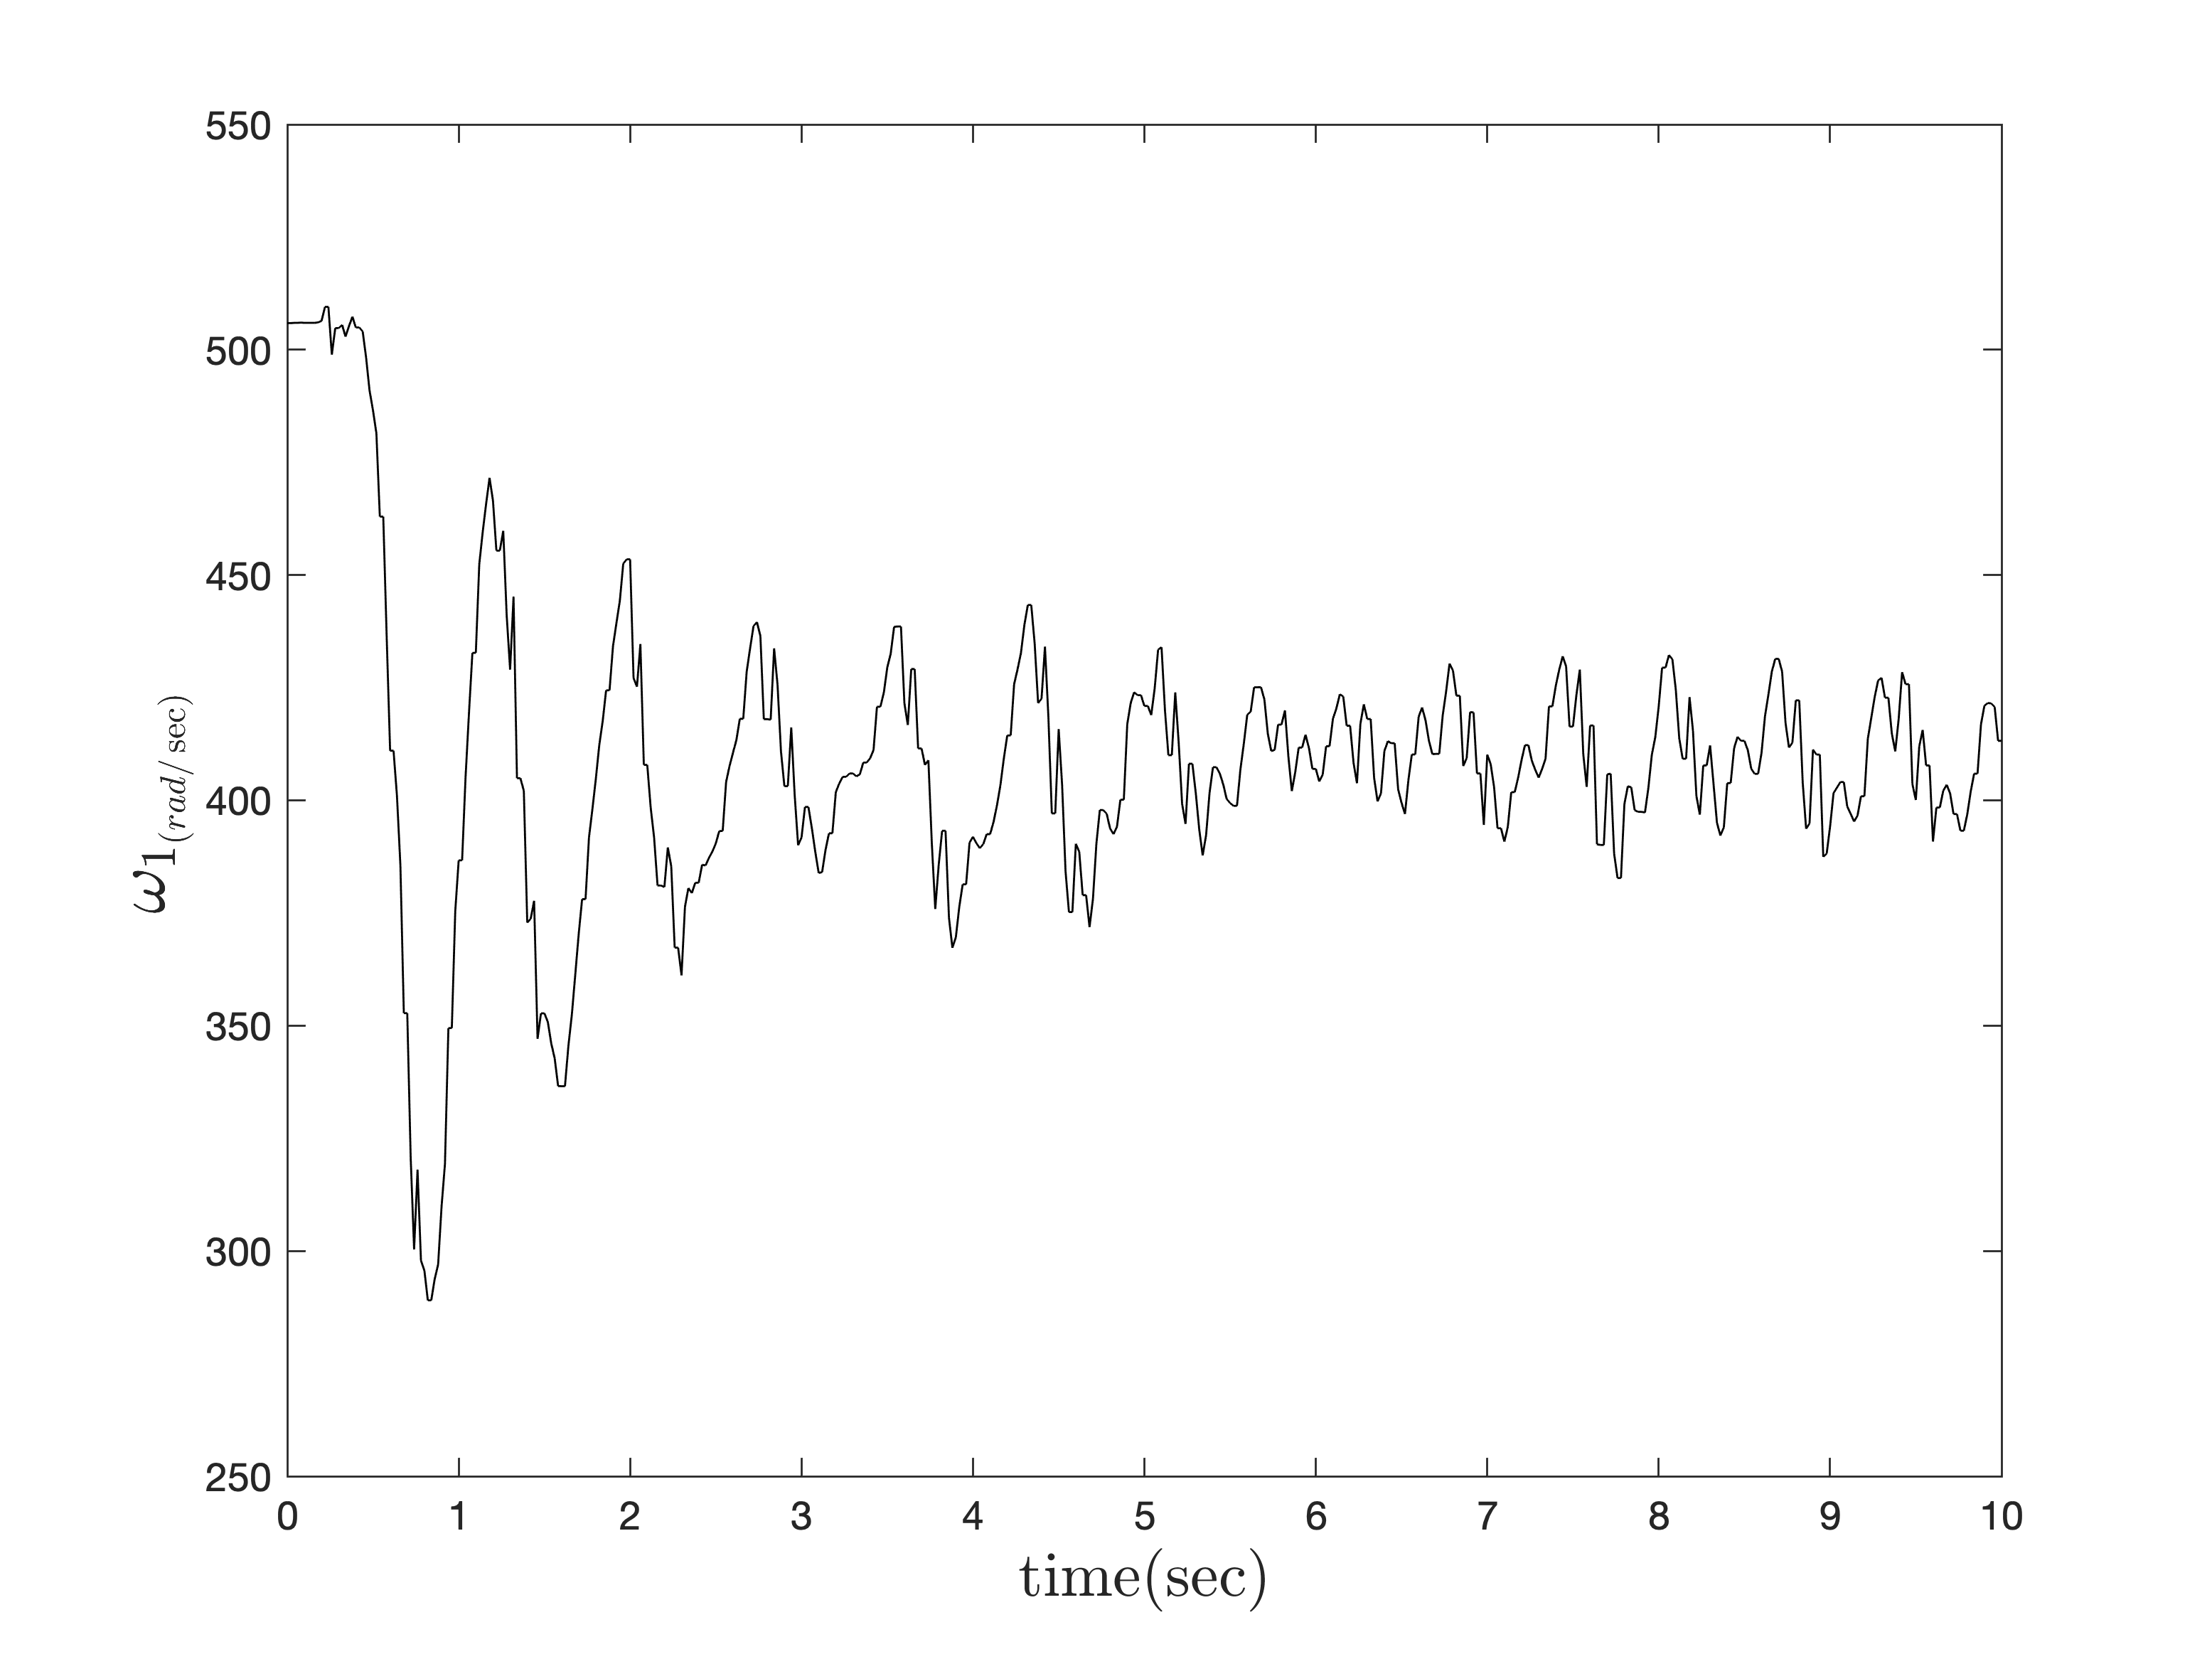
\includegraphics[width=.45\linewidth]{../Figures/Calibration/LQR/Pitch/lqr_pitch_Omega_1.png}
	}
	\subfigure[موتور شماره سه]{
		\centering
		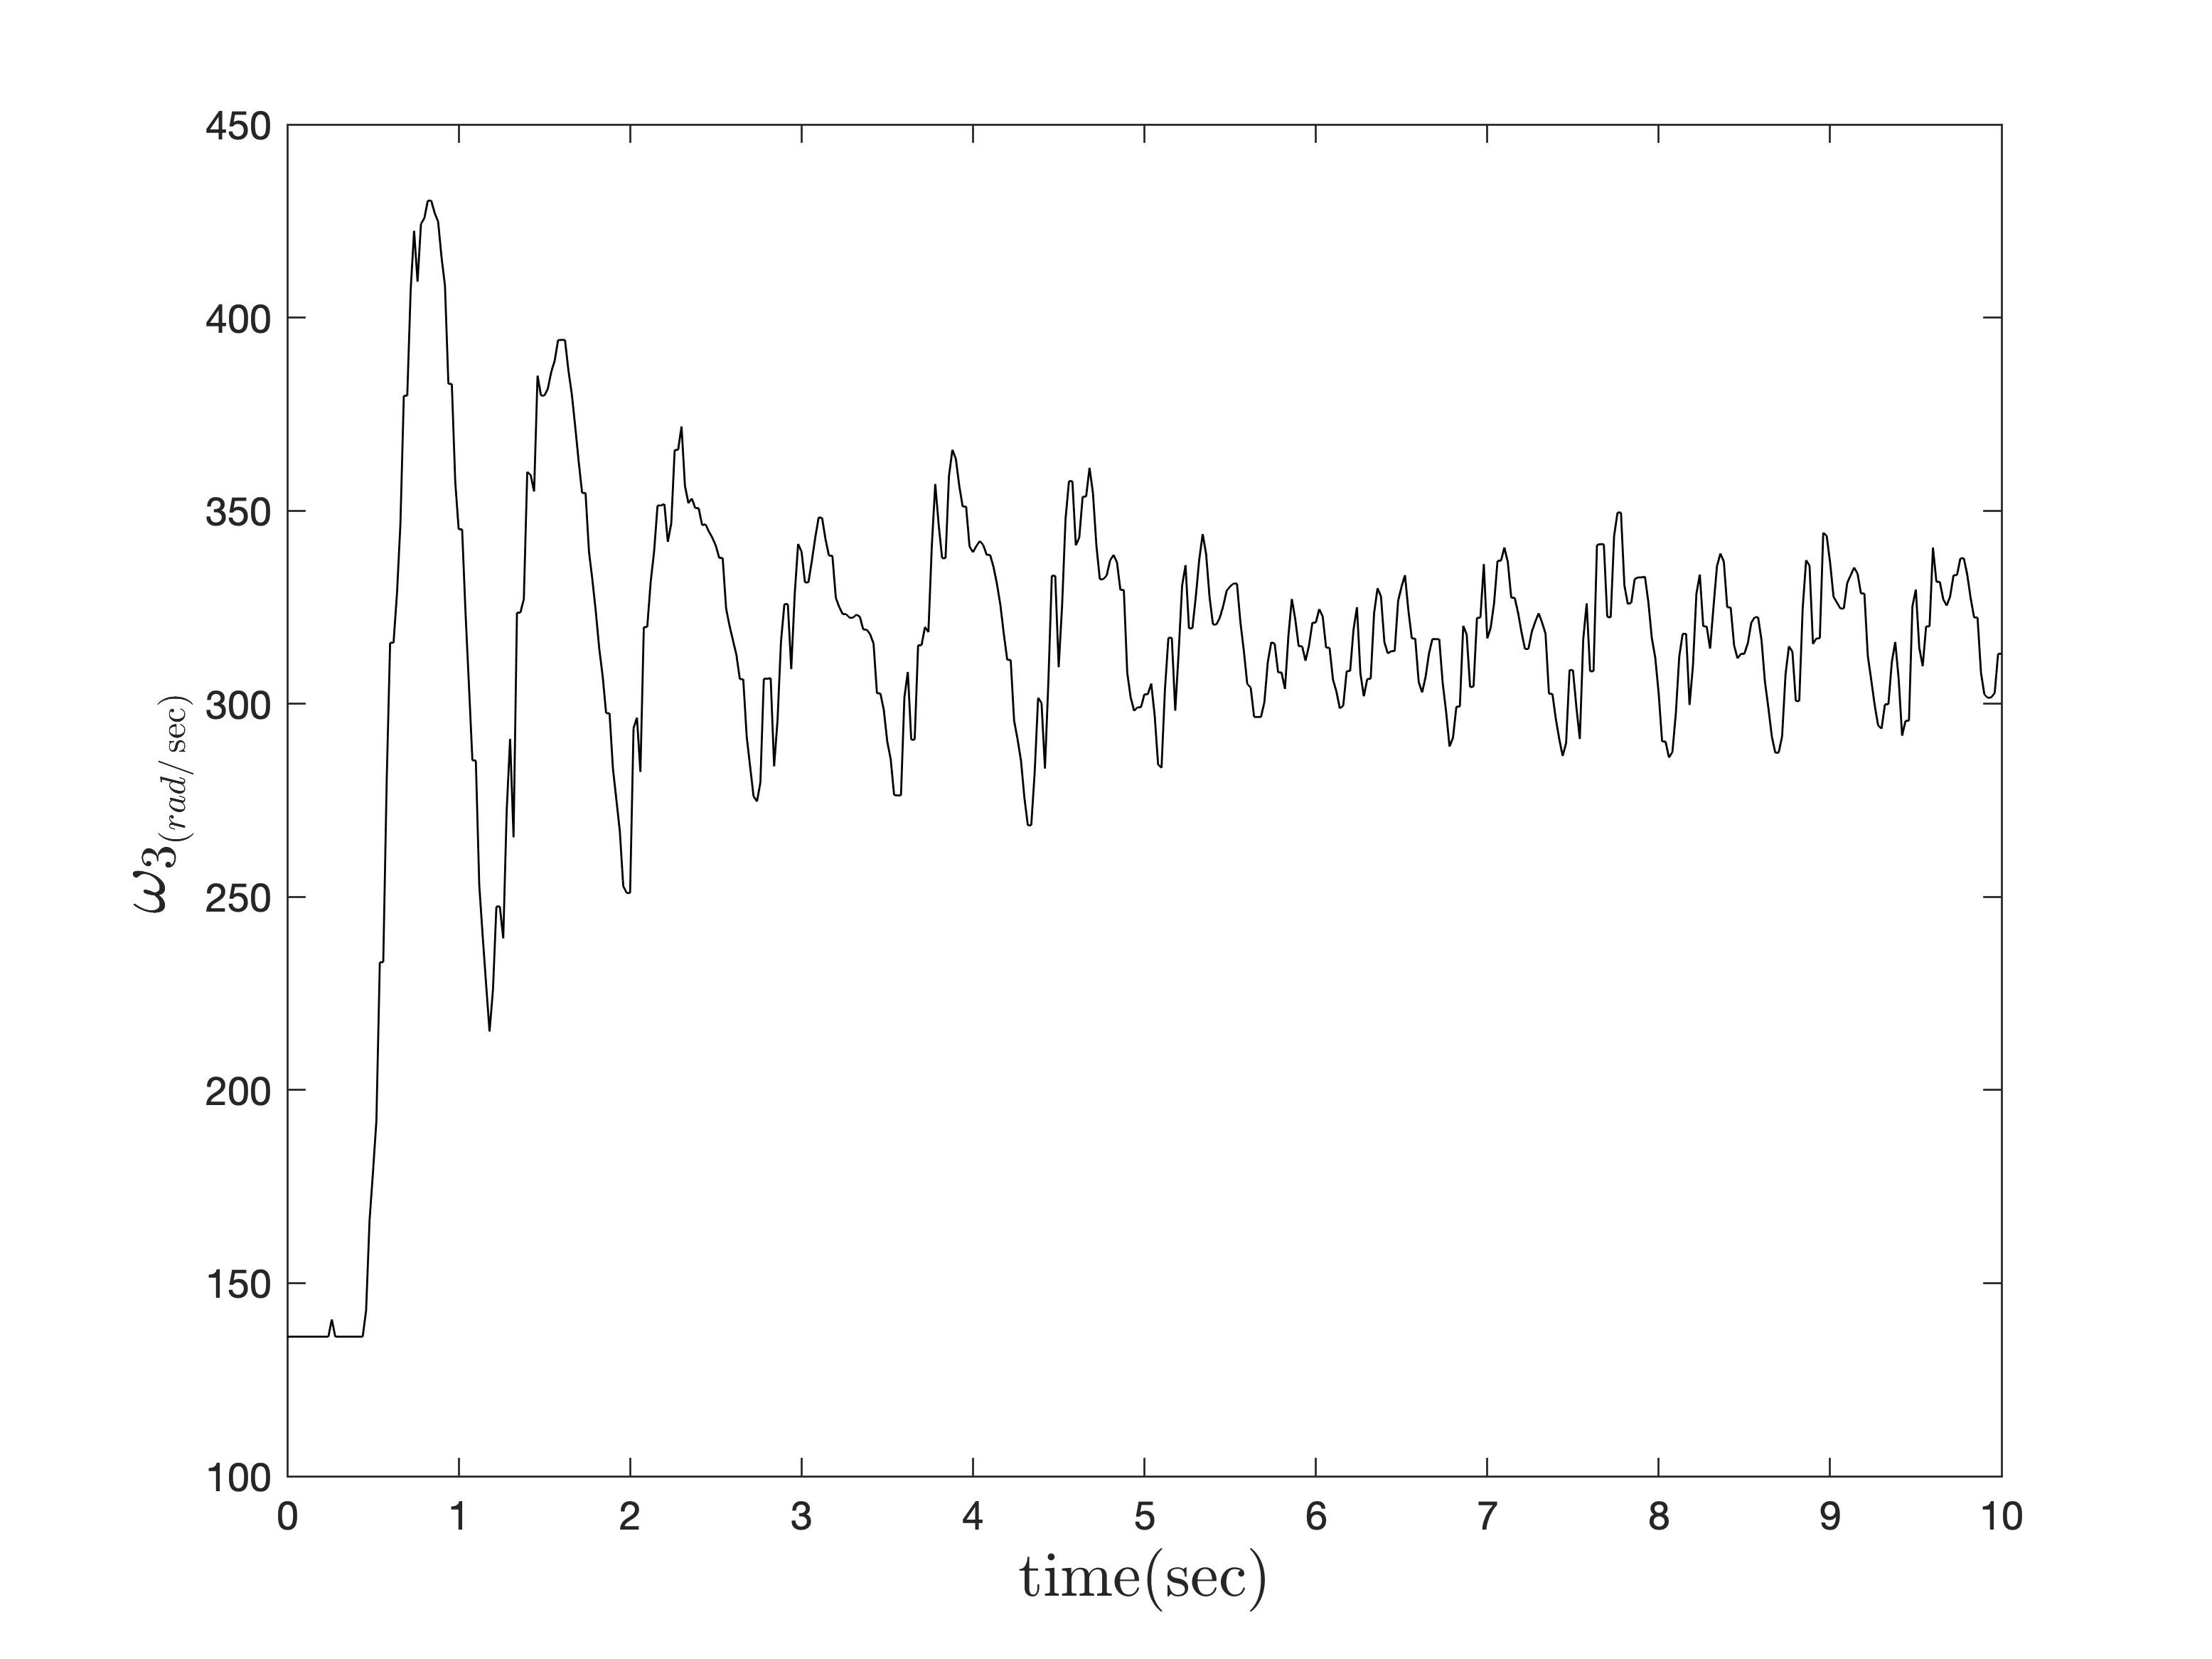
\includegraphics[width=.45\linewidth]{../Figures/Calibration/LQR/Pitch/lqr_pitch_Omega_3.png}
	}
	\caption{‫‪فرمان کنترلی موتورها در کنترل زاویه پیچ (تعقیب ورودی صفر)}
\end{figure}

بر اساس خروجی شبیه‌سازی (شکل
\ref{lqr_roll_fig})
،کانال رول در حضور کنترل‌کننده LQR در حدود پنج ثانیه به تعادل می‌رسد اما دارای خطای ماندگار است. 